\chapter{Kiểm thử và Đánh giá hệ thống}
\label{chap:testing}

Chương này trình bày các kịch bản kiểm thử thủ công (Manual Testing) nhằm đảm bảo các tính năng cốt lõi của ứng dụng MyBooksLibrary hoạt động đúng với yêu cầu đã đề ra. Đồng thời, chương cũng đưa ra những đánh giá khách quan về ưu, nhược điểm của phần mềm và đề xuất các hướng phát triển trong tương lai.

\section{Kịch bản kiểm thử (Manual Testing)}
Quá trình kiểm thử được thực hiện trực tiếp trên thiết bị di động thật (chạy hệ điều hành Android) nhằm đánh giá trải nghiệm thực tế của người dùng. Các bảng dưới đây trình bày kịch bản và kết quả kiểm thử cho 4 tính năng quan trọng nhất.

\subsection{Kiểm thử chức năng Khám phá và Tìm kiếm}
\begin{table}[H]
    \centering
    \caption{Kịch bản kiểm thử: Khám phá và Tìm kiếm truyện}
    \label{tab:test_discover}
    \begin{tabular}{|p{1.2cm}|p{3.2cm}|p{4.2cm}|p{3.5cm}|p{1.4cm}|}
    \hline
    \textbf{ID} & \textbf{Chức năng} & \textbf{Các bước thực hiện} & \textbf{Kết quả mong đợi} & \textbf{Kết quả} \\ \hline
    TC-01 & Tải danh sách truyện & Mở ứng dụng, chọn tab Khám phá. & Danh sách truyện hiển thị đầy đủ ảnh bìa và tên truyện nhanh chóng. & Pass \\ \hline
    TC-02 & Tìm kiếm truyện & Nhập từ khóa vào thanh tìm kiếm. & Hiển thị đúng các bộ truyện có chứa từ khóa vừa nhập. & Pass \\ \hline
    TC-03 & Lọc theo thể loại & Mở bộ lọc, chọn các thể loại tùy ý. & Chỉ hiển thị các bộ truyện thuộc các thể loại đã chọn. & Pass \\ \hline
    TC-04 & Cuộn trang vô tận & Cuộn xuống cuối danh sách truyện. & Tự động tải thêm (pagination) các bộ truyện tiếp theo mượt mà. & Pass \\ \hline
    \end{tabular}
\end{table}

\subsection{Kiểm thử chức năng Xem chi tiết và Đọc truyện}
\begin{table}[H]
    \centering
    \caption{Kịch bản kiểm thử: Xem chi tiết và Đọc truyện}
    \label{tab:test_read}
    \begin{tabular}{|p{1.2cm}|p{3.2cm}|p{4.2cm}|p{3.5cm}|p{1.4cm}|}
    \hline
    \textbf{ID} & \textbf{Chức năng} & \textbf{Các bước thực hiện} & \textbf{Kết quả mong đợi} & \textbf{Kết quả} \\ \hline
    TC-05 & Tải chi tiết truyện & Bấm vào 1 truyện từ danh sách. & Hiện thông tin tác giả, tóm tắt, và danh sách các chương. & Pass \\ \hline
    TC-06 & Load trang truyện & Chọn Chương 1 để bắt đầu đọc. & Ảnh trang truyện được tải lên đầy đủ, không bị vỡ hạt. & Pass \\ \hline
    TC-07 & Thao tác chuyển trang & Vuốt ngang/dọc trên màn hình. & Chuyển sang trang tiếp theo mượt mà, không giật lag. & Pass \\ \hline
    TC-08 & Lưu lịch sử đọc & Thoát ra khỏi chương đang đọc dở. & Hệ thống tự động ghi nhận chương và trang dừng lại cuối cùng. & Pass \\ \hline
    \end{tabular}
\end{table}

\subsection{Kiểm thử chức năng Quản lý Thư viện}
\begin{table}[H]
    \centering
    \caption{Kịch bản kiểm thử: Quản lý Thư viện cá nhân}
    \label{tab:test_library}
    \begin{tabular}{|p{1.2cm}|p{3.2cm}|p{4.2cm}|p{3.5cm}|p{1.4cm}|}
    \hline
    \textbf{ID} & \textbf{Chức năng} & \textbf{Các bước thực hiện} & \textbf{Kết quả mong đợi} & \textbf{Kết quả} \\ \hline
    TC-09 & Thêm vào Thư viện & Bấm nút "Lưu truyện" ở màn hình Chi tiết. & Biểu tượng đổi màu, truyện xuất hiện trong tab Thư viện. & Pass \\ \hline
    TC-10 & Xóa khỏi Thư viện & Bấm lại nút "Lưu truyện" (bỏ lưu). & Biểu tượng trở lại ban đầu, truyện biến mất khỏi tab Thư viện. & Pass \\ \hline
    TC-11 & Đồng bộ hóa đám mây & Đăng nhập Google, nhấn đồng bộ. & Lịch sử đọc và thư viện được đẩy lên/tải về từ Firebase. & Pass \\ \hline
    \end{tabular}
\end{table}

\subsection{Kiểm thử chức năng Tải xuống (Offline)}
\begin{table}[H]
    \centering
    \caption{Kịch bản kiểm thử: Tải truyện ngoại tuyến}
    \label{tab:test_download}
    \begin{tabular}{|p{1.2cm}|p{3.2cm}|p{4.2cm}|p{3.5cm}|p{1.4cm}|}
    \hline
    \textbf{ID} & \textbf{Chức năng} & \textbf{Các bước thực hiện} & \textbf{Kết quả mong đợi} & \textbf{Kết quả} \\ \hline
    TC-12 & Bắt đầu tải chương & Nhấn icon "Tải xuống" cạnh tên chương. & Thanh tiến trình xuất hiện, hiển thị \% hoàn thành. & Pass \\ \hline
    TC-13 & Đọc không cần mạng & Tắt Wi-Fi/4G, bấm vào chương đã tải. & Truyện vẫn mở lên và lướt qua được tất cả các trang bình thường. & Pass \\ \hline
    TC-14 & Quản lý dung lượng & Vào phần Quản lý tải xuống, xóa chương. & Dung lượng bộ nhớ được giải phóng, xóa ảnh khỏi thiết bị. & Pass \\ \hline
    \end{tabular}
\end{table}

\section{Kết quả kiểm thử trên giao diện thực tế}
Sau khi thực hiện các kịch bản kiểm thử, hệ thống ghi nhận ứng dụng hoạt động ổn định và đáp ứng đúng các luồng nghiệp vụ đề ra. Dưới đây là các ảnh chụp màn hình (screenshot) minh họa kết quả hiển thị trên thiết bị di động.

\begin{figure}[H]
    \centering
    % TODO: Chèn ảnh chụp màn hình Khám phá & Tìm kiếm
    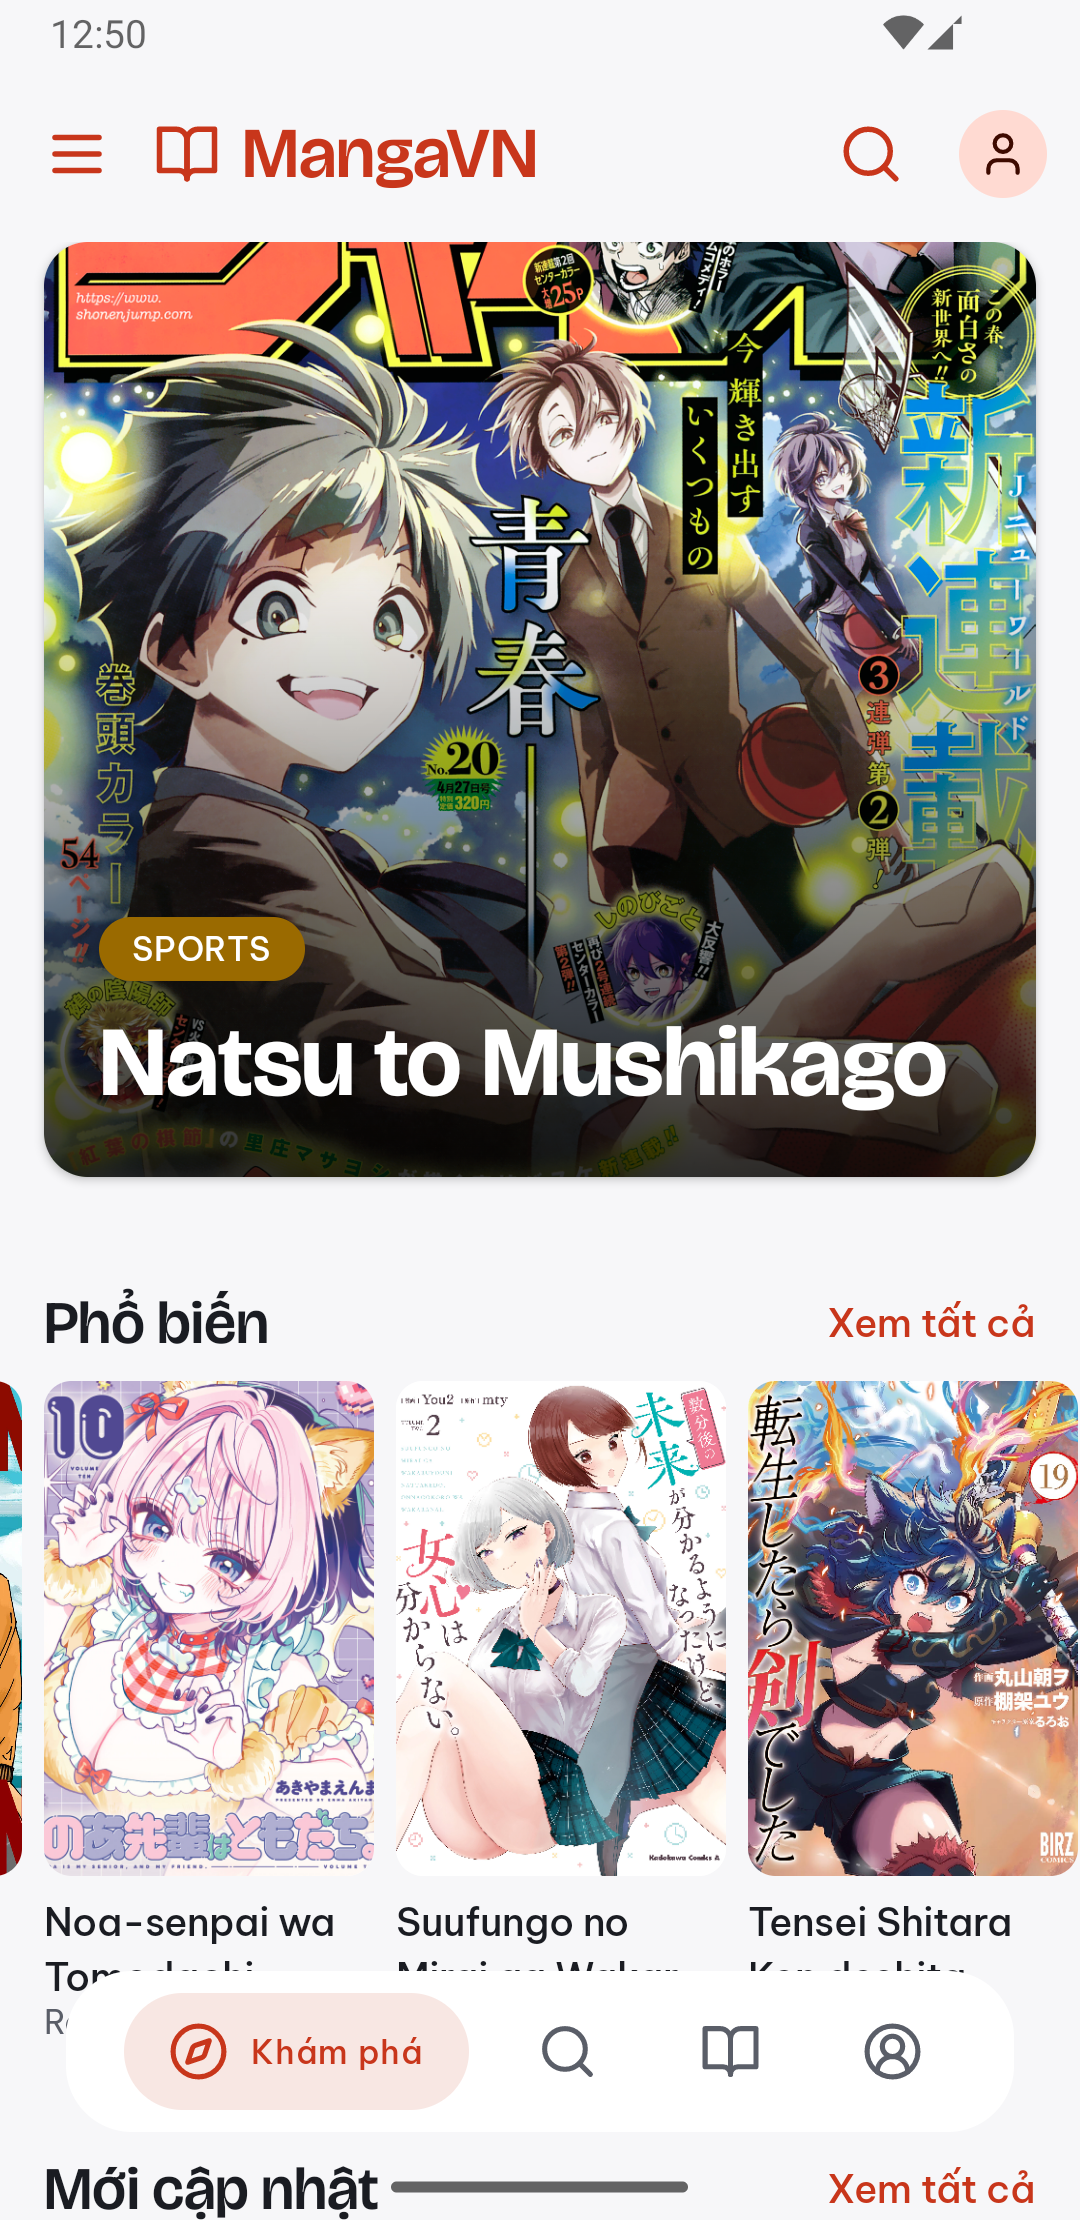
\includegraphics[width=0.45\textwidth]{figures/screenshot_discover.png}
    \hfill
    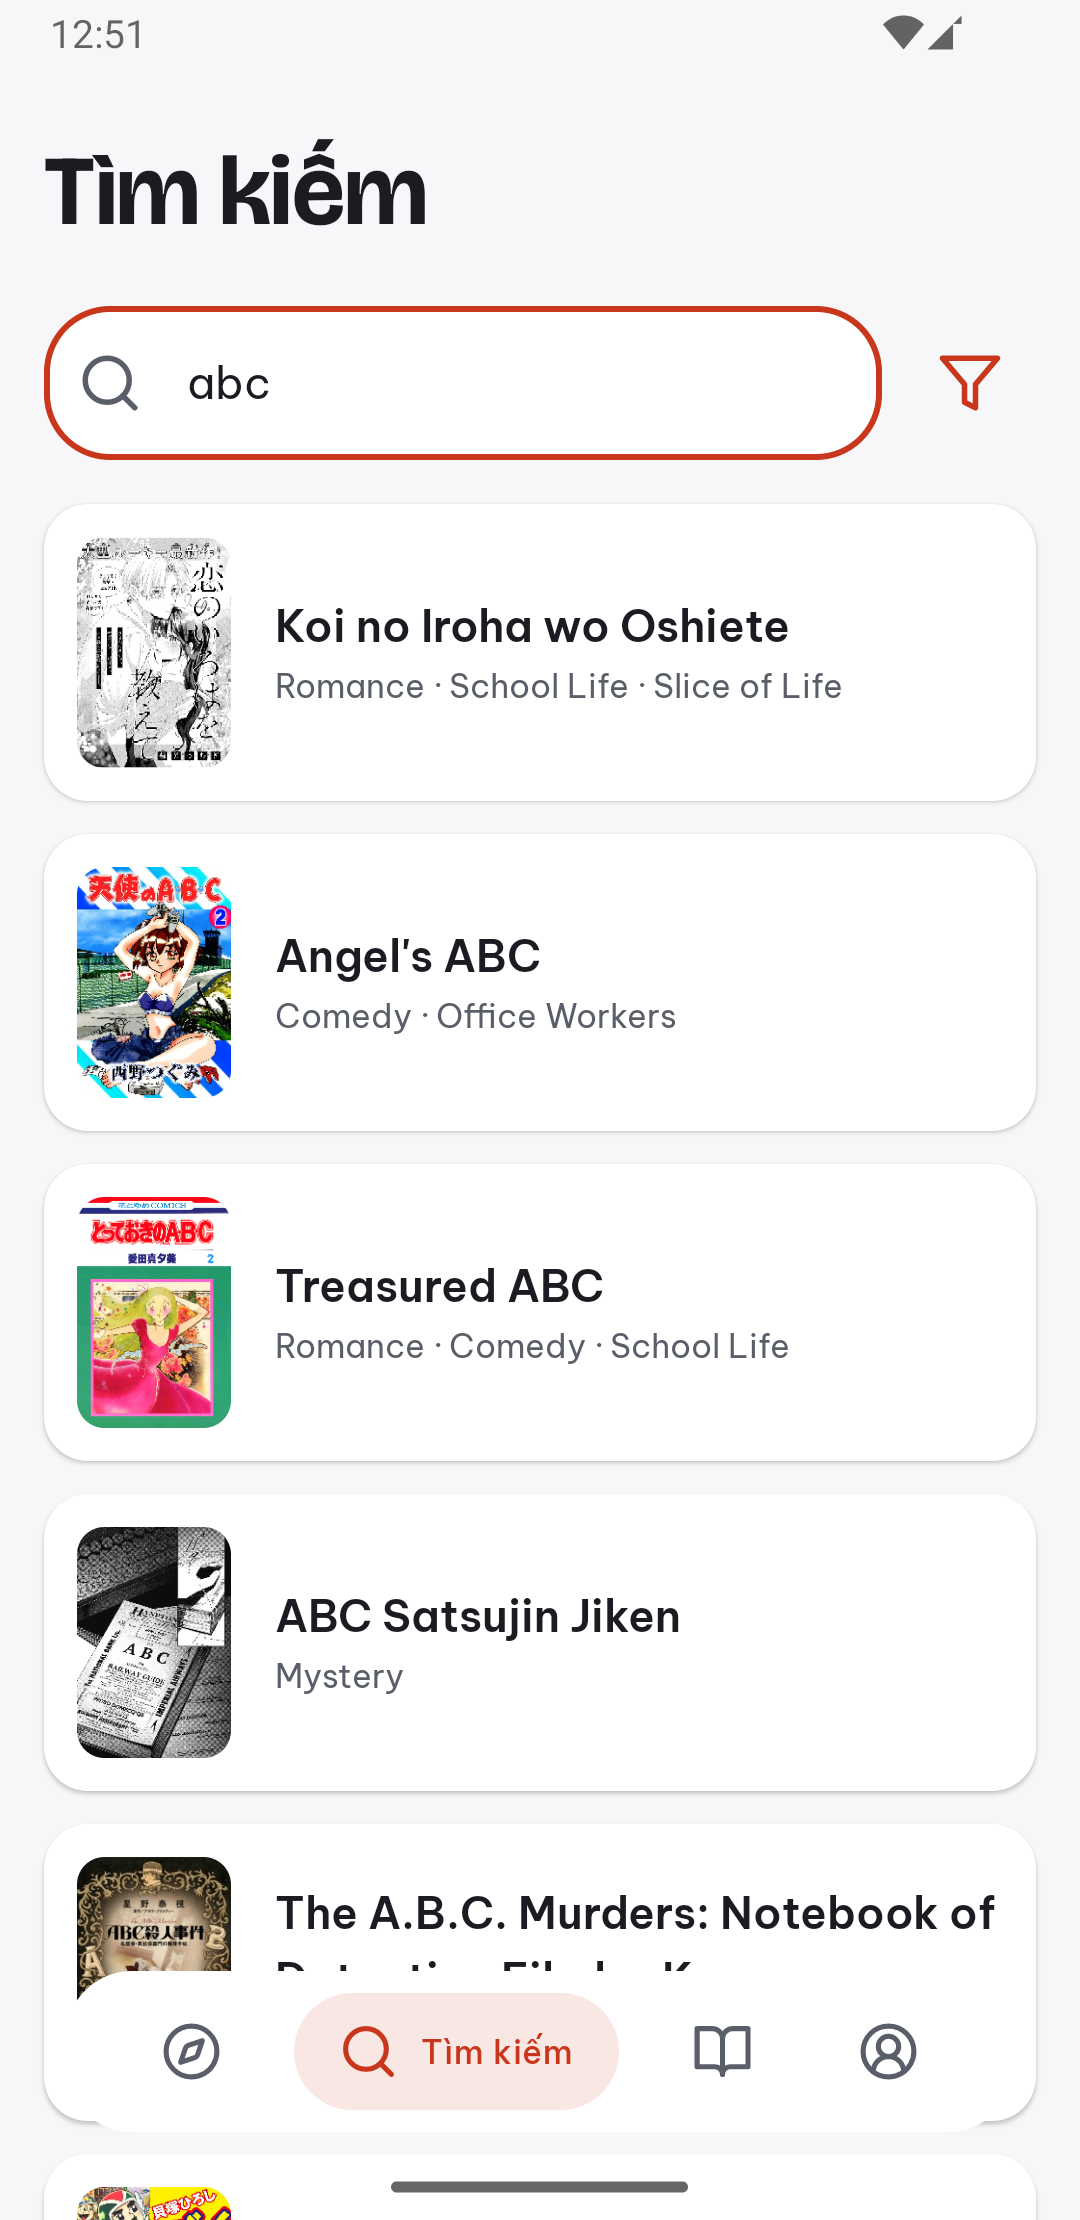
\includegraphics[width=0.45\textwidth]{figures/screenshot_search.png}
    \caption{Giao diện màn hình Khám phá (trái) và Tìm kiếm/Lọc truyện (phải)}
    \label{fig:res_discover}
\end{figure}

\begin{figure}[H]
    \centering
    % TODO: Chèn ảnh chụp màn hình Đọc truyện & Thư viện
    \includegraphics[width=0.45\textwidth]{figures/screenshot_reader.png}
    \hfill
    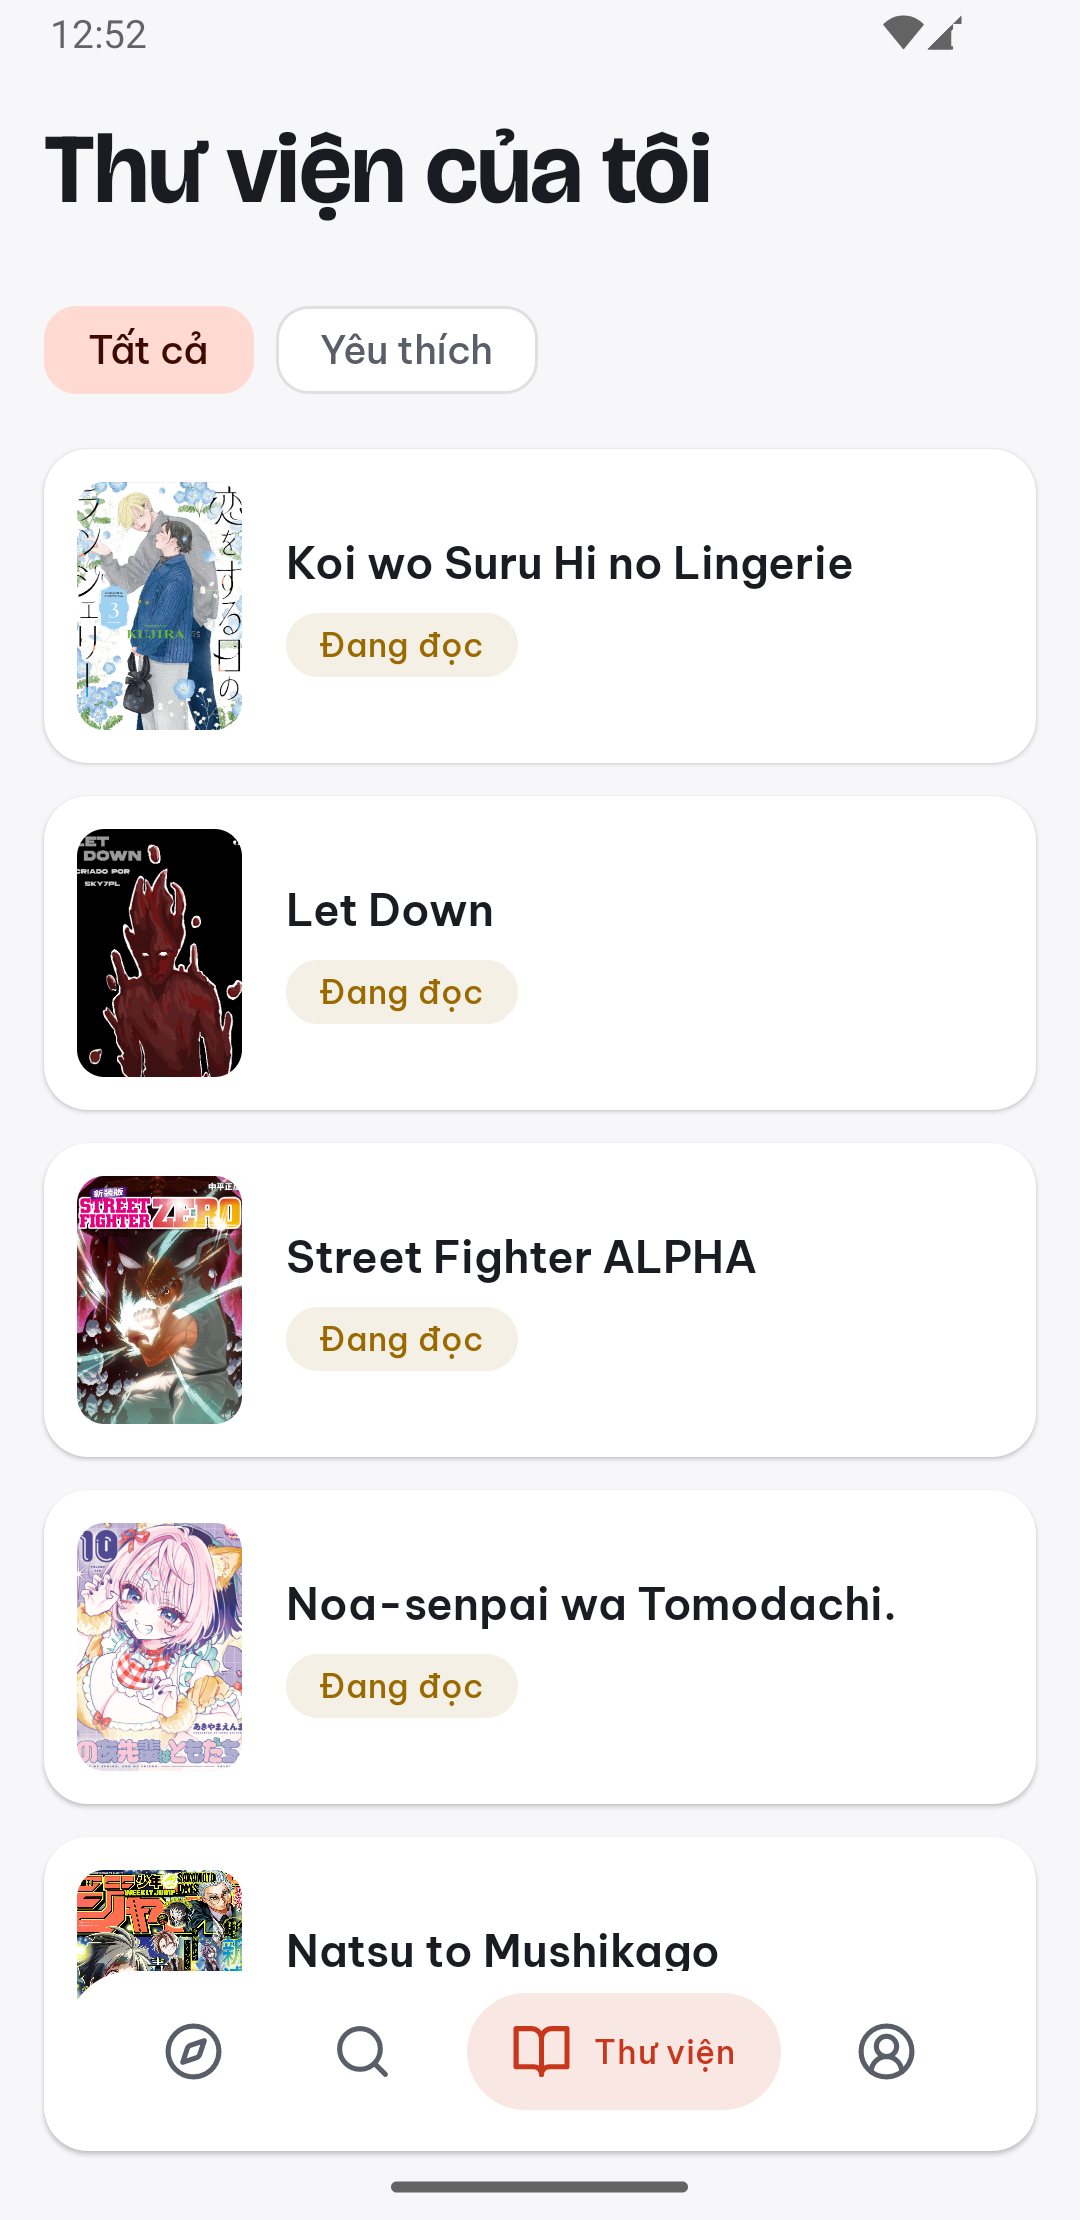
\includegraphics[width=0.45\textwidth]{figures/screenshot_library.png}
    \caption{Giao diện màn hình Đọc truyện (trái) và Thư viện cá nhân (phải)}
    \label{fig:res_reader}
\end{figure}

\section{Đánh giá ưu, nhược điểm của ứng dụng}
\subsection{Ưu điểm}
\begin{itemize}
    \item \textbf{Giao diện hiện đại, mượt mà:} Việc áp dụng Jetpack Compose và tiêu chuẩn Material Design 3 giúp ứng dụng có trải nghiệm tương tác (vuốt, chạm, chuyển cảnh) linh hoạt và đạt hiệu suất đồ họa cao.
    \item \textbf{Kiến trúc mở rộng tốt:} Tuân thủ Clean Architecture giúp tách biệt hoàn toàn logic nghiệp vụ với UI. Việc này hỗ trợ lập trình viên dễ dàng nâng cấp, thay thế một API cung cấp truyện khác trong tương lai mà không làm vỡ các thành phần hiện tại.
    \item \textbf{Tối ưu hoá đọc ngoại tuyến:} Hệ thống quản lý dữ liệu Room kết hợp với luồng tải bất đồng bộ giúp lưu trữ hình ảnh vật lý hiệu quả, giải quyết được bài toán đọc truyện khi mất kết nối mạng.
\end{itemize}

\subsection{Nhược điểm}
\begin{itemize}
    \item \textbf{Phụ thuộc nguồn dữ liệu duy nhất:} Ứng dụng hiện tại hoạt động dựa hoàn toàn vào API của MangaDex. Nếu hệ thống máy chủ này bảo trì hoặc thay đổi cấu trúc dữ liệu, toàn bộ ứng dụng sẽ bị tê liệt do không thể truy xuất nội dung.
    \item \textbf{Quản lý bộ nhớ Cache chưa triệt để:} Quá trình tải và hiển thị ảnh thông qua Coil sinh ra lượng lớn cache. Dù đem lại tốc độ mở truyện cực nhanh ở các lần đọc sau, nhưng nếu thiếu cơ chế dọn dẹp định kỳ thông minh, dung lượng ứng dụng có thể "phình" to ảnh hưởng tới thiết bị bộ nhớ thấp.
    \item \textbf{Thiếu tính năng tương tác xã hội:} Một ứng dụng đọc truyện lý tưởng cần có sự tương tác. Hiện tại người dùng chỉ có thể trải nghiệm cá nhân, chưa thể để lại bình luận, thảo luận hoặc chia sẻ trực tiếp với cộng đồng độc giả.
\end{itemize}

\section{Hướng phát triển tương lai}
Để khắc phục những hạn chế hiện có và nâng tầm chất lượng sản phẩm, các hướng phát triển trong thời gian tới được đề xuất bao gồm:
\begin{itemize}
    \item \textbf{Xây dựng kiến trúc Đa nguồn (Multi-source):} Bổ sung các module theo cơ chế Plugin để cho phép người dùng chuyển đổi lấy dữ liệu từ nhiều website/API truyện tranh khác nhau, giảm thiểu rủi ro khi một server nguồn bị sập.
    \item \textbf{Phát triển tính năng cộng đồng:} Xây dựng một Backend Server trung gian (Node.js/Spring Boot) hoặc mở rộng Firebase để hỗ trợ hệ thống bình luận (Comment), diễn đàn thu nhỏ và tính năng đánh giá (Rating) cho từng bộ truyện.
    \item \textbf{Hệ thống gợi ý thông minh (Recommendation System):} Áp dụng các mô hình học máy (Machine Learning) cơ bản để phân tích sở thích, thói quen đọc truyện của từng cá nhân, từ đó tự động đưa ra các đề xuất truyện phù hợp.
    \item \textbf{Tối ưu hóa quản lý dung lượng tự động:} Tích hợp tính năng tự dọn dẹp các ảnh cache đã lưu quá 30 ngày, hoặc đề xuất người dùng tự xóa các chương truyện tải xuống sau khi đọc xong.
\end{itemize}